% !TEX encoding = UTF-8 Unicode
% -*- coding: UTF-8; -*-
% vim: set fenc=utf-8


\subsection{Klientská část komponenty}\label{subsec:klientskáČást}

Klientská část komponenty musí komunikovat se zvoleným textovým editorem, zachytávat uživatelský vstup a následně ho převést na abstraktní object operace, který lze dále použít v rámci algoritmu \gls{OT}.
Tato část také musí umět komunikovat pomocí zvolené komunikační technologie s částí serverovou (z důvodu propagace jednotlivých Operací mezi uživateli).

Struktura klientské části je znázorněna pomocí třídního diagramu na obrázku~\ref{fig:EditorClient}.
Jádrem celé části je třída \texttt{EditorClient}, která dědí od třídy \texttt{Client} z knihovny OT.js.
Dědí vlastnosti a metody implementující jádro algoritmu \gls{OT}, jako je například udržování čísla revize a transformace přijatých operací v případě existence nepotvrzené vlastní operace.
Třída \texttt{Client} a tedy i třída \texttt{EditorClient} je navržena podle návrhového vzoru stav, který je popsán v~\cite[str.~283]{gof:patterns}, a může nabývat 3 stavů (viz stavový diagram na obrázku~\ref{fig:stavovyDiagram}).

\begin{figure}[ht!]
    \centering
    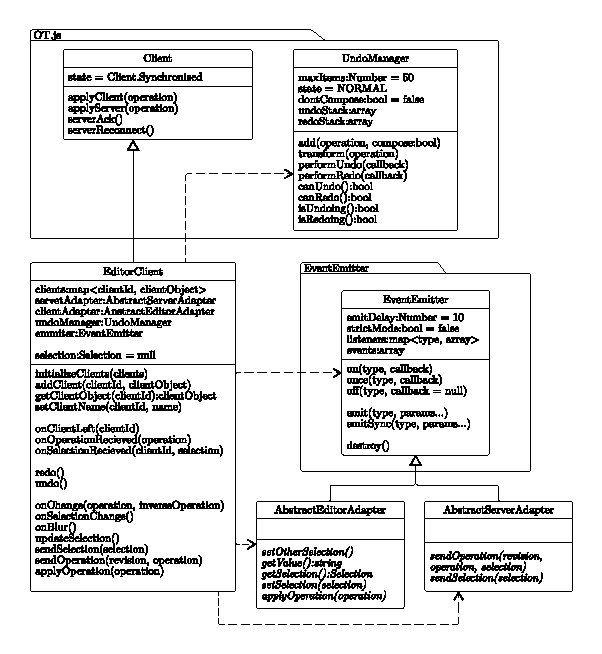
\includegraphics[width=\textwidth]{partials/navrh/editor/EditorClient.pdf}
    \caption{Třídní diagram klientské části komponenty}\label{fig:EditorClient}
\end{figure}

\begin{figure}[ht!]
    \centering
    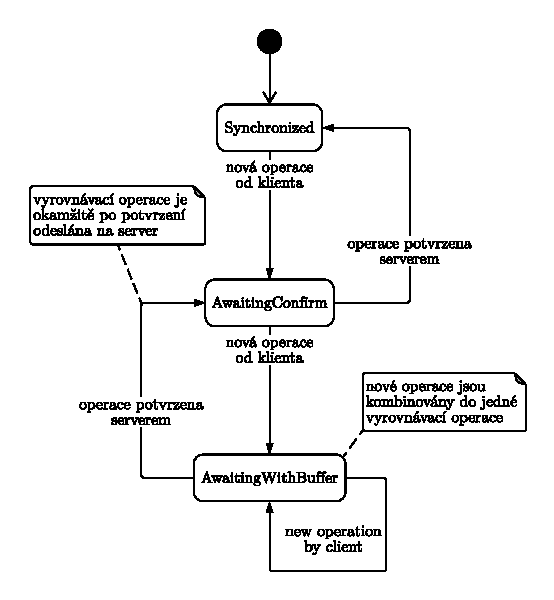
\includegraphics[width=\textwidth]{partials/navrh/editor/stavovyDiagram.pdf}
    \caption{Stavový diagram klientské části komponenty}\label{fig:stavovyDiagram}
\end{figure}

Třída \texttt{EditorClient} očekává implementaci třídy \texttt{AbstractEditorAdapter} (respektive \texttt{AbstractServerAdapter}), která slouží jako rozhraní pro komunikaci s textovým editorem (respektive serverovou částí).
Tyto třídy jsou navrženy podle návrhového vzoru adaptér, tak jak je popsán v~\cite[str.~135]{gof:patterns}, a umožňují spolupráci rozdílných rozhraní (například rozhraní textového editoru a třídy \texttt{EditorClient}).
Použití abstraktních tříd umožňuje změnu jednotlivých částí aplikace (například změna komunikační technologie, či knihovny textového editoru) a to bez nutnosti zásahu do logiky synchronizace samotných textů.

Tyto abstraktní třídy jsou také potomky třídy \texttt{EventEmitter}, která je ustálenou a rozšířenou implementací návrhového vzoru Pozorovatel (anglicky Observer)~\cite[str.~273]{gof:patterns} pro jazyk Javascript.
Rozhraní \texttt{EventEmitter} umožňuje třídě \texttt{EditorClient} naslouchat jednotlivým událostem, ke kterým dochází v implementacích zmíněných abstraktních tříd (jako je například změna pozice kursoru, či přijatá operace od serveru).
Seznam jednotlivých událostí je možné pozorovat na diagramu~\ref{fig:AbstractEditorAdapter} (respektive~\ref{fig:AbstractServerAdapter}).

\begin{figure}[ht!]
    \centering
    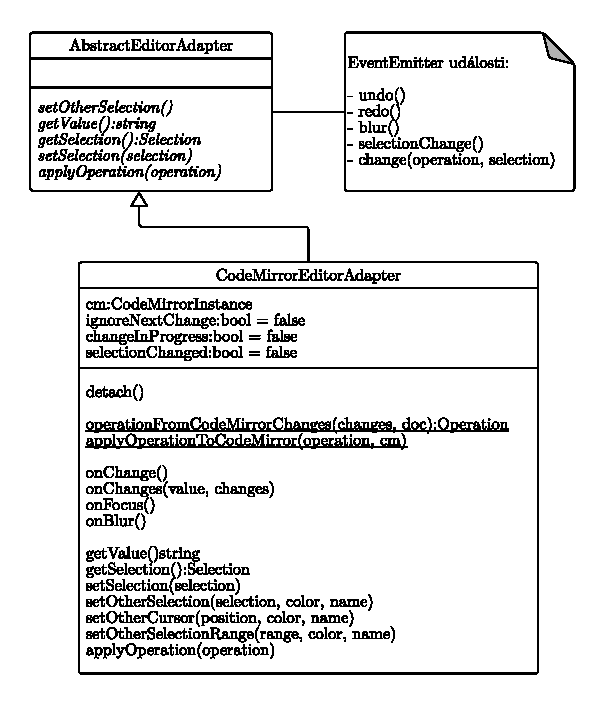
\includegraphics[width=.8\textwidth]{partials/navrh/editor/AbstractEditorAdapter.pdf}
    \caption{Diagram implementace třídy AbstractEditorAdapter}\label{fig:AbstractEditorAdapter}
\end{figure}

\begin{figure}[ht!]
    \centering
    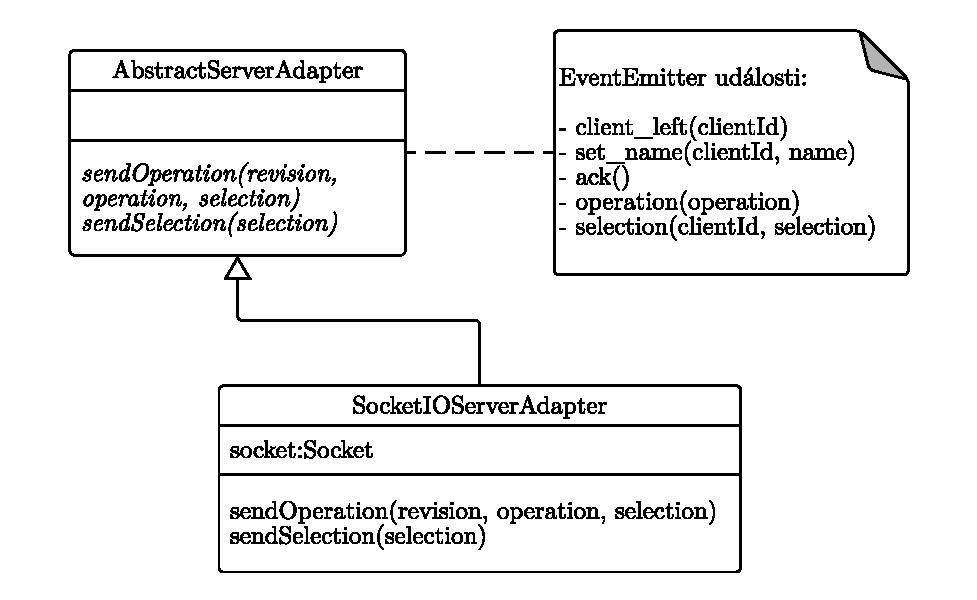
\includegraphics[width=.8\textwidth]{partials/navrh/editor/AbstractServerAdapter.pdf}
    \caption{Diagram implementace třídy AbstractServerAdapter}\label{fig:AbstractServerAdapter}
\end{figure}

\texttt{EditorClient} také využívá třídu \texttt{UndoManager} z knihovny OT.js, díky které lze bezpečně použít funkce zpět a vykonat znovu (pokud jejich odchycení podporuje poskytnutá implementace třídy \texttt{AbstractEditorAdapter}).
Historie je zaznamenávána pomocí jednotlivých operací vykonaných uživatelem a nikoliv podle změn samotného textu, jak by tomu bylo běžně.
Na změnách textu se totiž může podílet více uživatelů najednou a je nežádoucí, aby například funkce zpět vracela i změny provedené jiným než lokálním uživatelem.

% !TEX encoding = UTF-8 Unicode
% -*- coding: UTF-8; -*-
% vim: set fenc=utf-8

\subsubsection{React rozhraní komponenty}

Klientská část komponenty v prototypu je zapouzdřena do React komponenty (více o knihovně React v sekci~\ref{subsec:reactjs}) pojmenované \texttt{RealtimeEditor}.
React komponenta umožňuje klientskou část znovu použít kdekoliv v aplikaci a pomocí modulárního návrhu lze upravit i její vzhled.

React komponenta po svém prvním vykreslení vytvoří spojení k serverové části a vytvoří instanci textového editoru CodeMirror.
Ty následně předá nově vytvořeným instancím tříd \texttt{SocketIOServerAdapter} a \texttt{CodeMirrorEditorAdapter}.
Komponenta dále vytvoří instanci třídy \texttt{EditorClient}, které předá vytvořené instance tříd \texttt{SocketIOServerAdapter} a \texttt{CodeMirrorEditorAdapter}.
Komponenta ve svém stavu drží informace o připojených klientech, nastavení a další informace ohledně aktuálně připojeného dokumentu.

React komponenta \texttt{RealtimeEditor} přijímá jak povinné, tak i nepovinné vlastnosti (viz tabulka~\ref{tab:reactKomponenta}).

\begin{table}[ht!]\centering
\caption{Vlastnosti přijímané React komponentou RealtimeEditor}\label{tab:reactKomponenta}

\begin{tabular}{l c c p{5.5cm}}
    Jméno: & Povinná: & Datový typ: & Popis:\\ \hline
    documentId & ano & String & Identifikátor dokumentu\\ \hline
    user & ne & Object & Informace o přihlášeném uživateli\\ \hline
    headerSlot & ne & Node & Komponenta vykreslená na místě hlavičky dokumentu \\ \hline
    menuSlot & ne & Node & Komponenta vykreslená na místě menu dokumentu \\ \hline
    errorSlot & ne & Node & Komponenta vykreslená pokud dojde k chybě \\
\end{tabular}
\end{table}

Vlastnost \texttt{documentId} označuje identifikátor dokumentu, ke kterému se komponenta má připojit.
Vlastnost \texttt{user} je objekt s informacemi o přihlášeném uživateli (očekávaná struktura je stejná jako struktura získaná pomocí \gls{REST} koncového bodu~\ref{subsubsec:GET/api/user}).
V případě nepřihlášeného uživatele není nutné vlastnost \texttt{user} vůbec předávat, či lze předat libovolnou hodnotu, která se vyhodnotí jako nepravda.
Poslední vlastnosti \texttt{headerSlot}, \texttt{menuSlot} a \texttt{errorSlot} označují modulární React komponenty vykreslené na specifickém místě \texttt{RealtimeEditor} komponenty.
Modulárním komponentám jsou předány vnitřní informace o stavu editoru pomocí jejich vlastností a jsou tak upozorněny i v případě jejich změny.

Nejjednodušší použití komponenty je ukázané ve výpisu kódu~\ref{lst:RealtimeEditor}.
Tento příklad vykreslí pouze samotný textový editor, který je ovšem aktualizovaný v reálném čase se všemi uživateli, kteří jsou ve stejnou chvíli připojeni k dokumentu s identifikátorem \enquote{helloWorld}.

\begin{listing}[ht!]
    \begin{minted}{javascript}
        export default () => (
            <RealtimeEditor documentId="helloWorld"/>
        )
    \end{minted}

    \caption{Příklad použití komponenty RealtimeEditor}\label{lst:RealtimeEditor}
\end{listing}

